\chapter{Gradients of all architectures - gradually shifted}\label{appendixC}

\section*{Velocity - Full dataset}\label{sec:velocity-appendixC}

\begin{figure}[!htpb]
\centering
\begin{subfigure}[b]{\textwidth}
   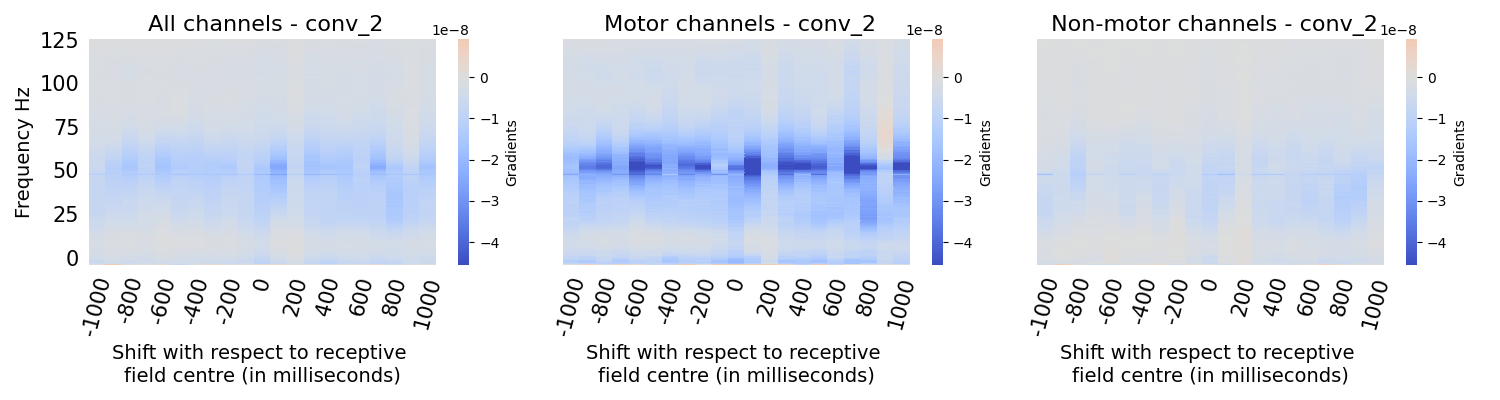
\includegraphics[width=1\linewidth]{img/appendix/C/m/vel/sbp0_m_shift_gradients_conv_2_all_kinds}
   \caption{}
   \label{fig:vel-shifting-grads-conv-2}
\end{subfigure}

\begin{subfigure}[b]{\textwidth}
   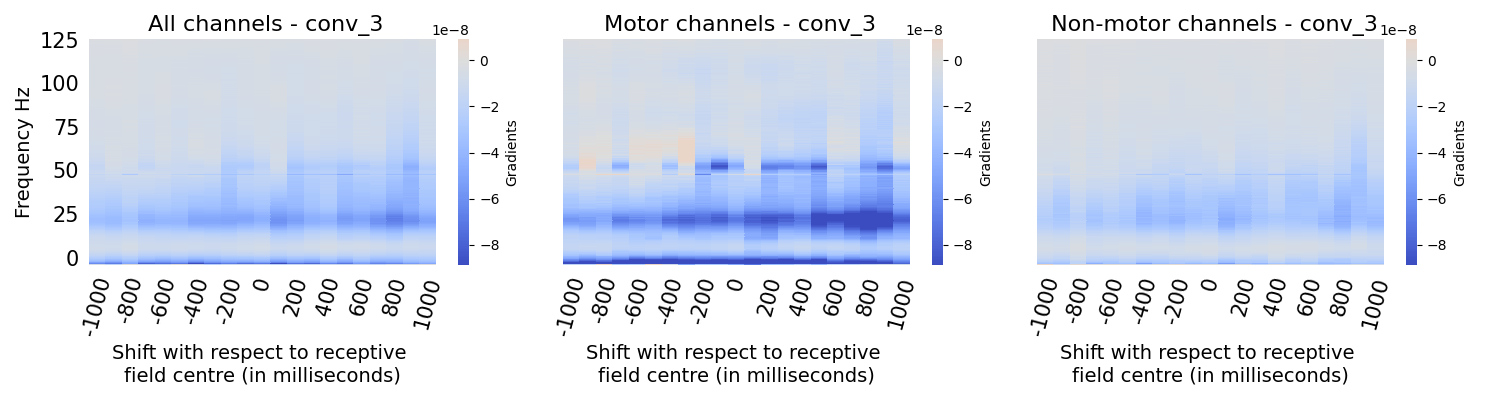
\includegraphics[width=1\linewidth]{img/appendix/C/m/vel/sbp0_m_shift_gradients_conv_3_all_kinds}
   \caption{}
   \label{fig:vel-shifting-grads-conv-3}
\end{subfigure}
\end{figure}
\clearpage
\begin{figure}
\ContinuedFloat

\begin{subfigure}[b]{\textwidth}
   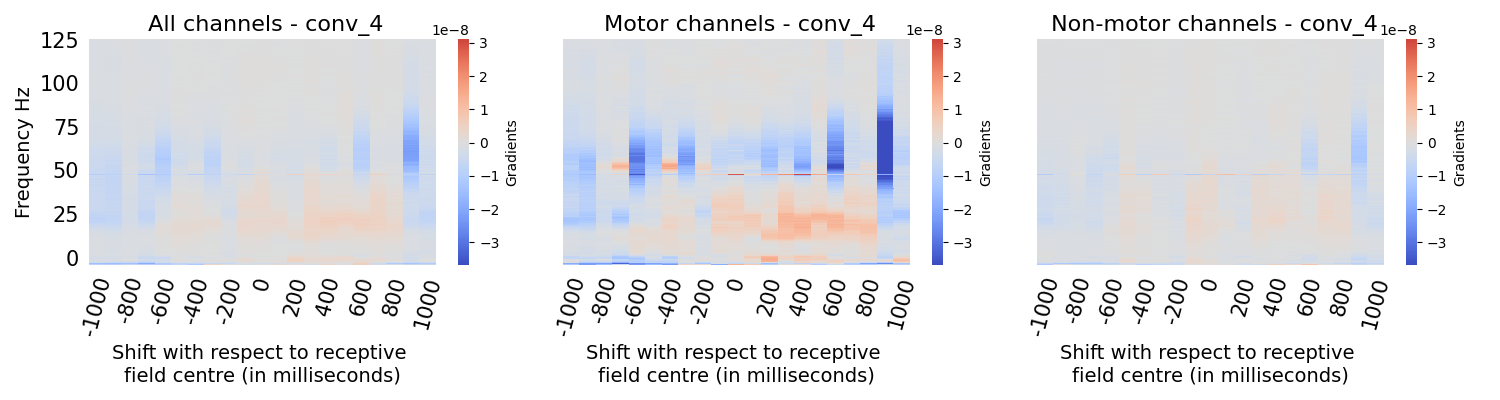
\includegraphics[width=1\linewidth]{img/appendix/C/m/vel/sbp0_m_shift_gradients_conv_4_all_kinds}
   \caption{}
   \label{fig:vel-shifting-grads-conv-4}
\end{subfigure}

\begin{subfigure}[b]{\textwidth}
   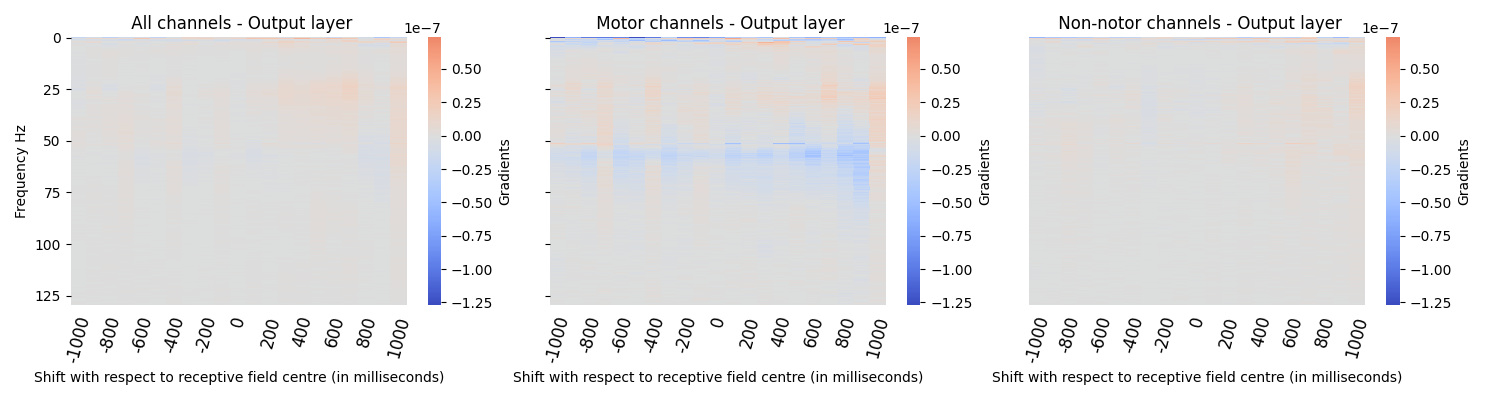
\includegraphics[width=1\linewidth]{img/appendix/C/m/vel/sbp0_m_shift_gradients_conv_classifier_all_kinds}
   \caption{}
   \label{fig:vel-shifting-grads-conv-classifier}
\end{subfigure}

\caption[]{Gradients of the different CNN architectures decoding velocity from the full dataset when gradually shifting the predicted time-point (see Section~\ref{subsec:shifting-the-predicted-time-point-across-receptive-field}. \textbf{(a)} shows gradients of the convolutional layer in the second block; \textbf{(b)} shows gradients of the convolutional layer in the third block; \textbf{(c)} shows gradients of the fourth convolutional block; \textbf{(d)} shows gradients of the last convolutional layer - the output layer. All channels include channels that do not belong to motor neither non-motor channel sets. See Section \ref{subsec:ieeg-data-preprocessing}}
\label{fig:vel-shifting-grads}
\end{figure}

\clearpage
\section*{Velocity - High-passed dataset}\label{subsec:vel-high-passed-dataset-appendixC}
\begin{figure}[!htpb]
\centering
\begin{subfigure}[b]{\textwidth}
   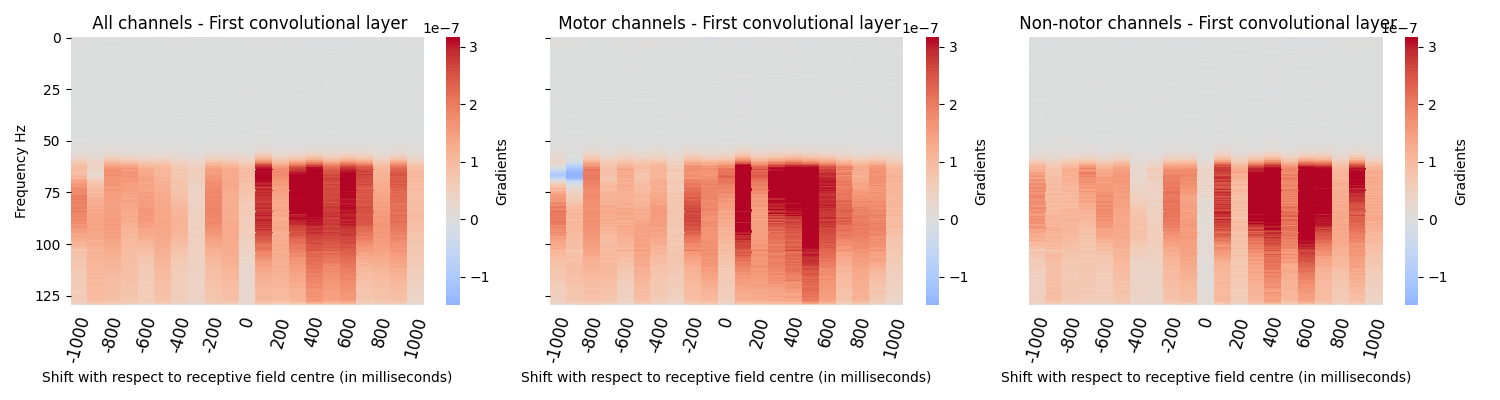
\includegraphics[width=0.85\linewidth]{img/appendix/C/hp-m/vel/sbp0_hp_m_shift_gradients_conv_2_all_kinds}
   \caption{}
   \label{fig:vel-hp-shifting-grads-conv-2}
\end{subfigure}

\begin{subfigure}[b]{\textwidth}
   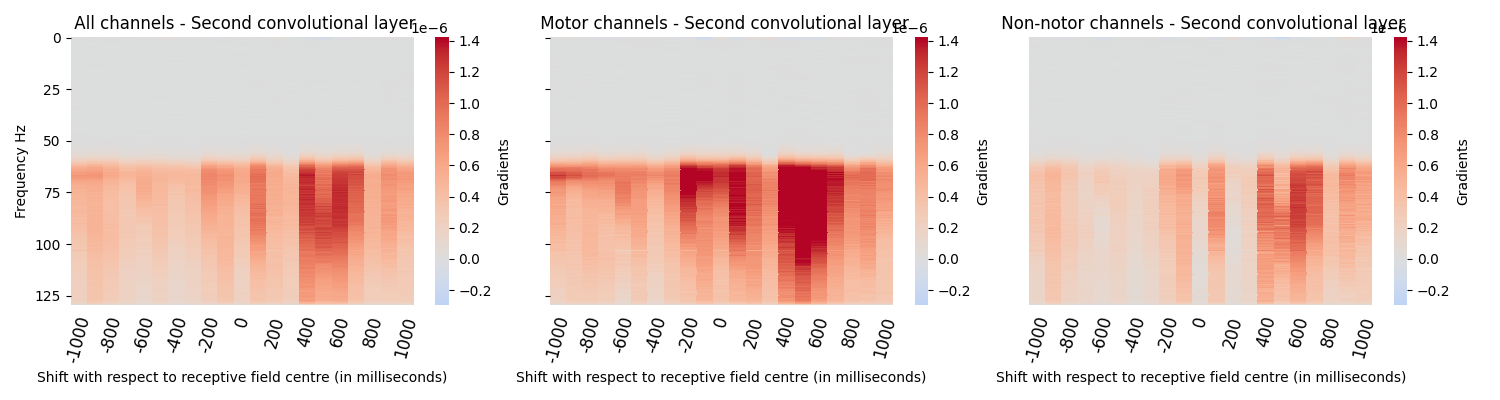
\includegraphics[width=0.85\linewidth]{img/appendix/C/hp-m/vel/sbp0_hp_m_shift_gradients_conv_3_all_kinds}
   \caption{}
   \label{fig:vel-hp-shifting-grads-conv-3}
\end{subfigure}

\begin{subfigure}[b]{\textwidth}
   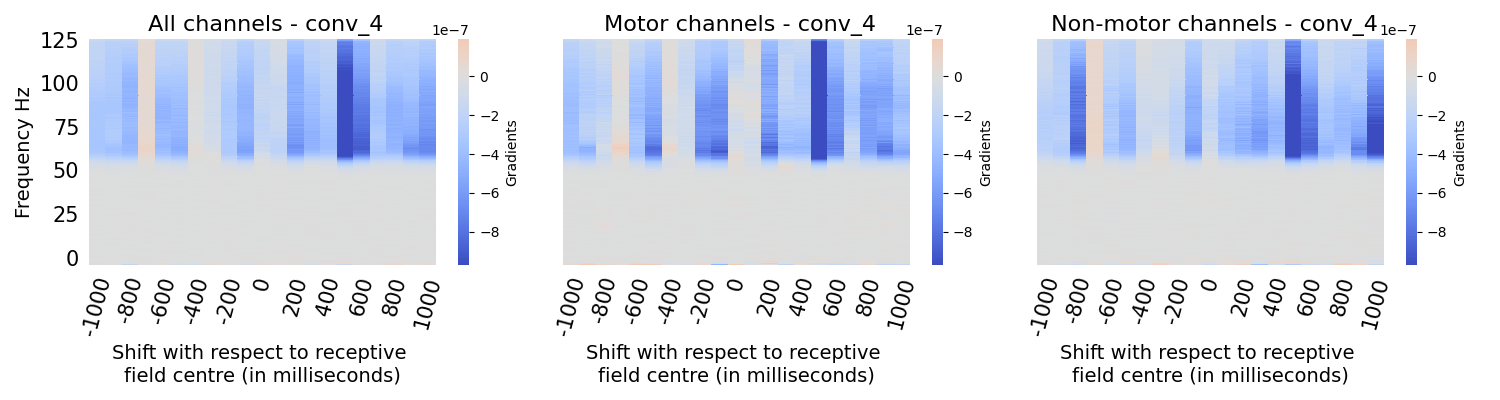
\includegraphics[width=0.85\linewidth]{img/appendix/C/hp-m/vel/sbp0_hp_m_shift_gradients_conv_4_all_kinds}
   \caption{}
   \label{fig:vel-hp-shifting-grads-conv-4}
\end{subfigure}

\begin{subfigure}[b]{\textwidth}
   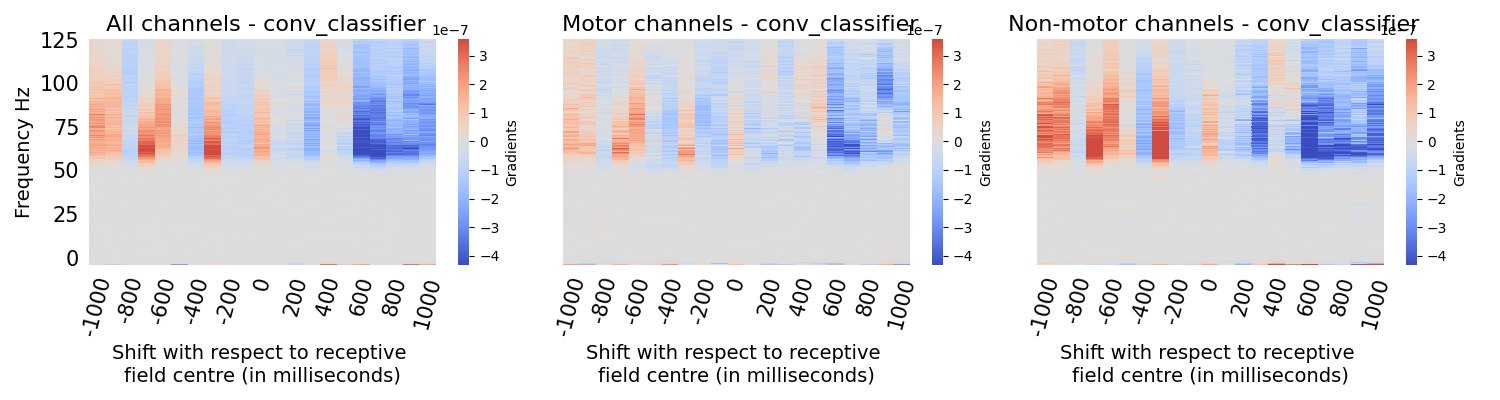
\includegraphics[width=0.85\linewidth]{img/appendix/C/hp-m/vel/sbp0_hp_m_shift_gradients_conv_classifier_all_kinds}
   \caption{}
   \label{fig:vel-hp-shifting-grads-conv-classifier}
\end{subfigure}

\caption[]{Gradients of the different CNN architectures decoding velocity from the high-passed dataset when gradually shifting the predicted time-point (see Section~\ref{subsec:shifting-the-predicted-time-point-across-receptive-field}. \textbf{(a)} shows gradients of the convolutional layer in the second block; \textbf{(b)} shows gradients of the convolutional layer in the third block; \textbf{(c)} shows gradients of the fourth convolutional block; \textbf{(d)} shows gradients of the last convolutional layer - the output layer. All channels include channels that do not belong to motor neither non-motor channel sets. See Section \ref{subsec:ieeg-data-preprocessing}}
\label{fig:vel-hp-shifting-grads}
\end{figure}
\clearpage
\section*{Absolute velocity - Full dataset}\label{sec:absolute-velocity-appendixC}

\begin{figure}[!htpb]
\centering
\begin{subfigure}[b]{\textwidth}
   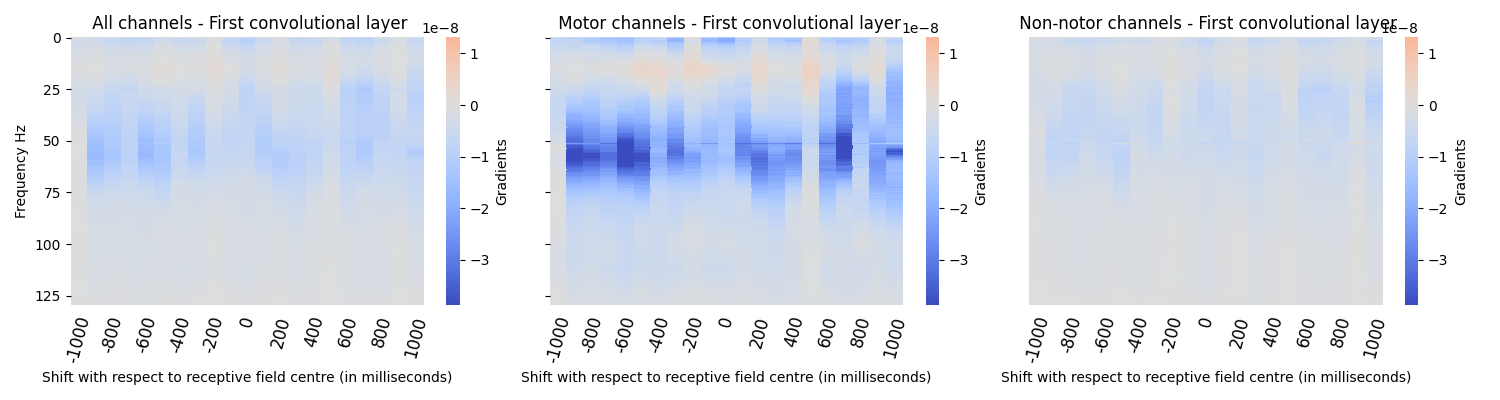
\includegraphics[width=0.85\linewidth]{img/appendix/C/m/absVel/sbp0_m_shift_gradients_conv_2_all_kinds}
   \caption{}
   \label{fig:absVel-shifting-grads-conv-2}
\end{subfigure}

\begin{subfigure}[b]{\textwidth}
   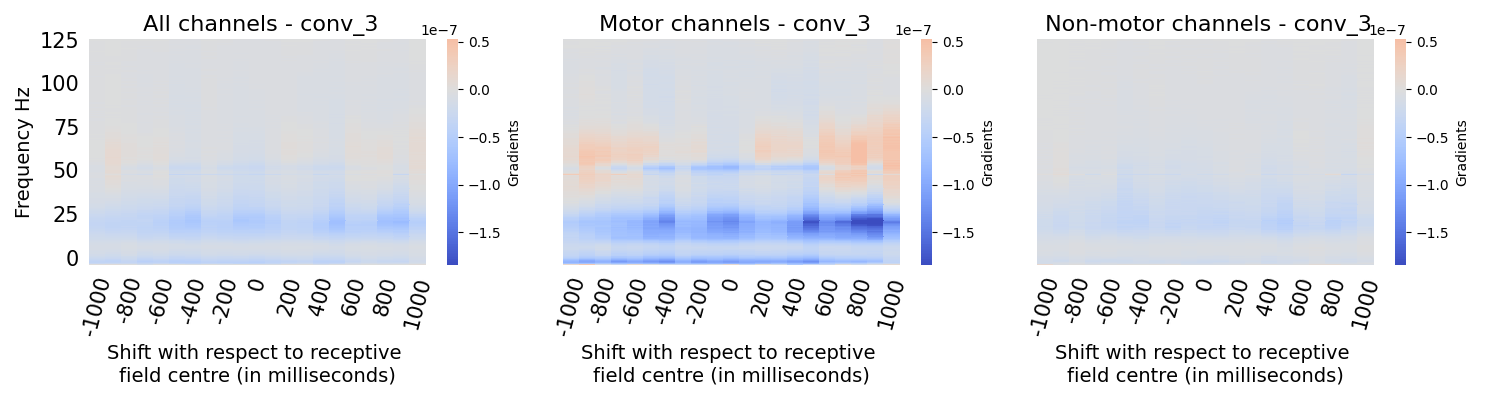
\includegraphics[width=0.85\linewidth]{img/appendix/C/m/absVel/sbp0_m_shift_gradients_conv_3_all_kinds}
   \caption{}
   \label{fig:absVel-shifting-grads-conv-3}
\end{subfigure}

\begin{subfigure}[b]{\textwidth}
   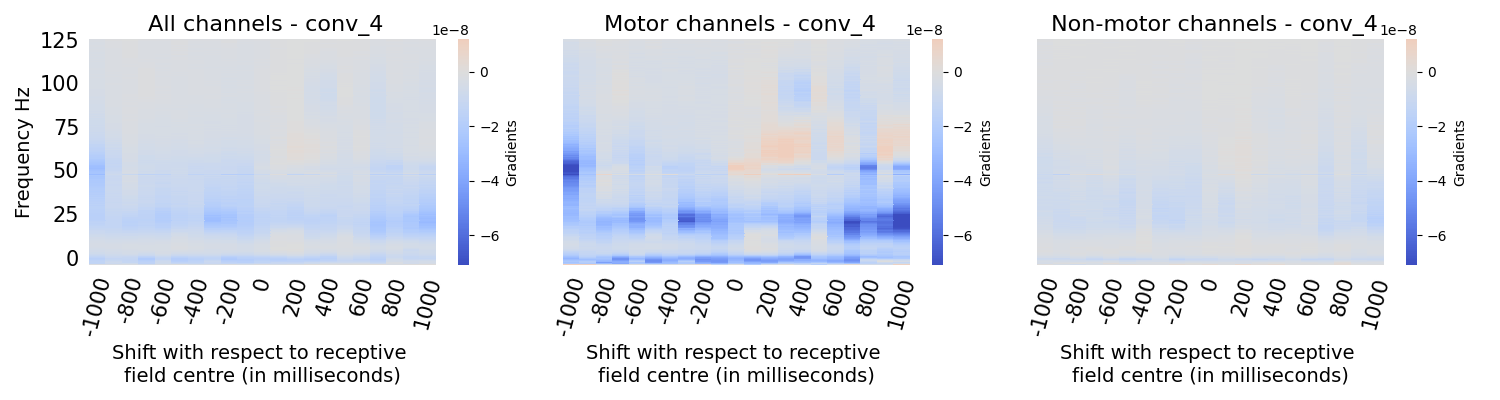
\includegraphics[width=0.85\linewidth]{img/appendix/C/m/absVel/sbp0_m_shift_gradients_conv_4_all_kinds}
   \caption{}
   \label{fig:absVel-shifting-grads-conv-4}
\end{subfigure}

\begin{subfigure}[b]{\textwidth}
   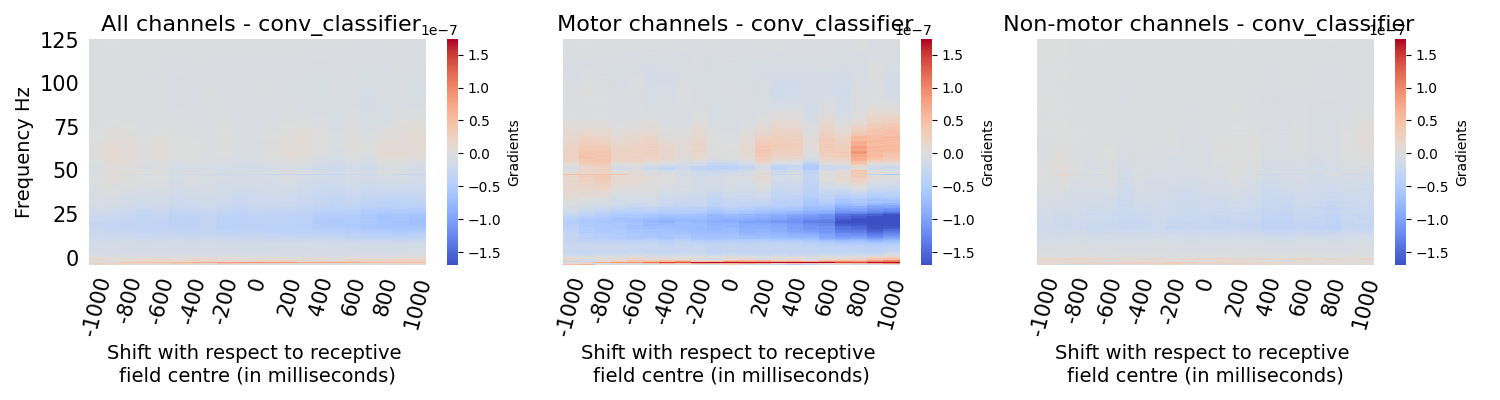
\includegraphics[width=0.85\linewidth]{img/appendix/C/m/absVel/sbp0_m_shift_gradients_conv_classifier_all_kinds}
   \caption{}
   \label{fig:absVel-shifting-grads-conv-classifier}
\end{subfigure}

\caption[]{Gradients of the different CNN architectures decoding absolute velocity from the full dataset when gradually shifting the predicted time-point (see Section~\ref{subsec:shifting-the-predicted-time-point-across-receptive-field}. \textbf{(a)} shows gradients of the convolutional layer in the second block; \textbf{(b)} shows gradients of the convolutional layer in the third block; \textbf{(c)} shows gradients of the fourth convolutional block; \textbf{(d)} shows gradients of the last convolutional layer - the output layer. All channels include channels that do not belong to motor neither non-motor channel sets. See Section \ref{subsec:ieeg-data-preprocessing}}
\label{fig:absVel-shifting-grads}
\end{figure}

\clearpage
\section*{Absolute velocity - High-passed dataset}\label{subsec:absVel-high-passed-dataset-appendixC}
\begin{figure}[!htpb]
\centering
\begin{subfigure}[b]{\textwidth}
   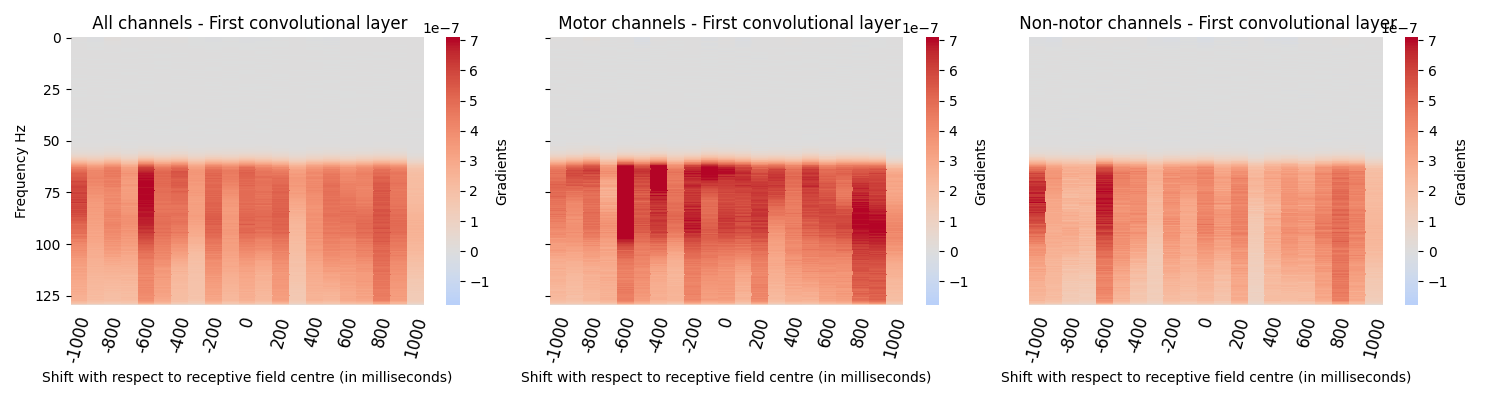
\includegraphics[width=0.85\linewidth]{img/appendix/C/hp-m/absVel/sbp0_hp_m_shift_gradients_conv_2_all_kinds}
   \caption{}
   \label{fig:absVel-hp-shifting-grads-conv-2}
\end{subfigure}

\begin{subfigure}[b]{\textwidth}
   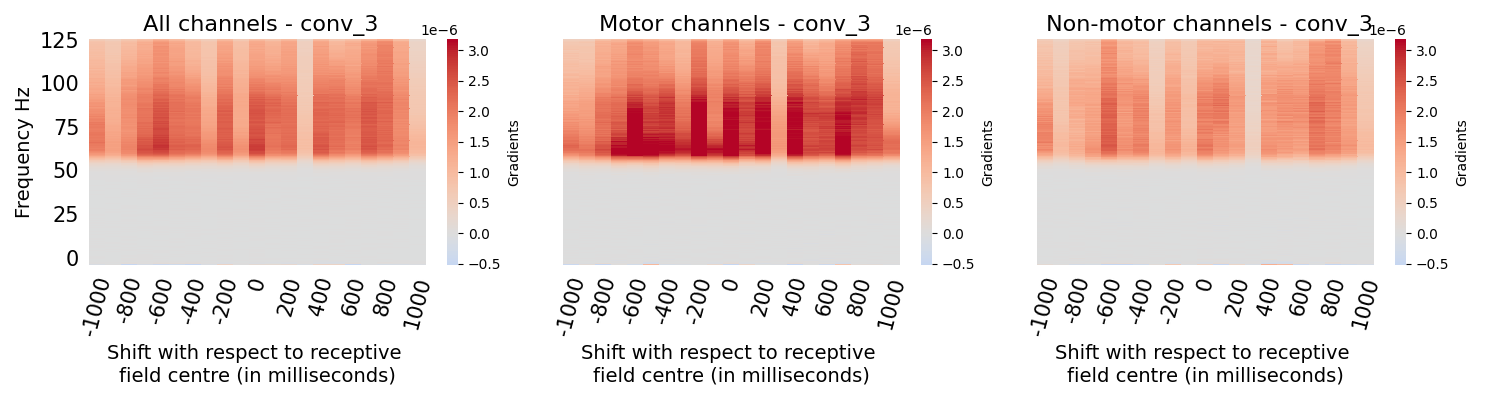
\includegraphics[width=0.85\linewidth]{img/appendix/C/hp-m/absVel/sbp0_hp_m_shift_gradients_conv_3_all_kinds}
   \caption{}
   \label{fig:absVel-hp-shifting-grads-conv-3}
\end{subfigure}

\begin{subfigure}[b]{\textwidth}
   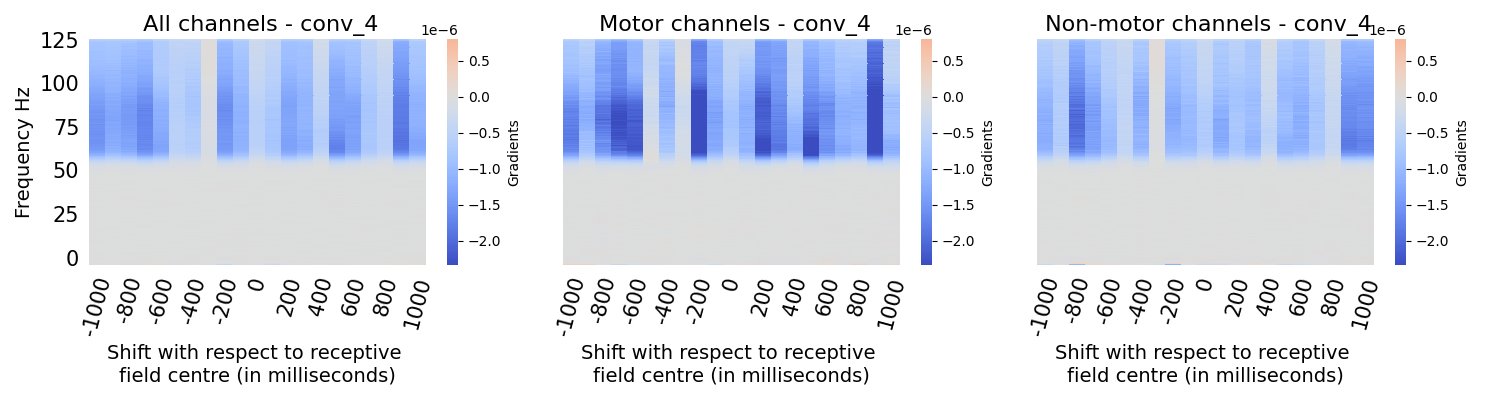
\includegraphics[width=0.85\linewidth]{img/appendix/C/hp-m/absVel/sbp0_hp_m_shift_gradients_conv_4_all_kinds}
   \caption{}
   \label{fig:absVel-hp-shifting-grads-conv-4}
\end{subfigure}

\begin{subfigure}[b]{\textwidth}
   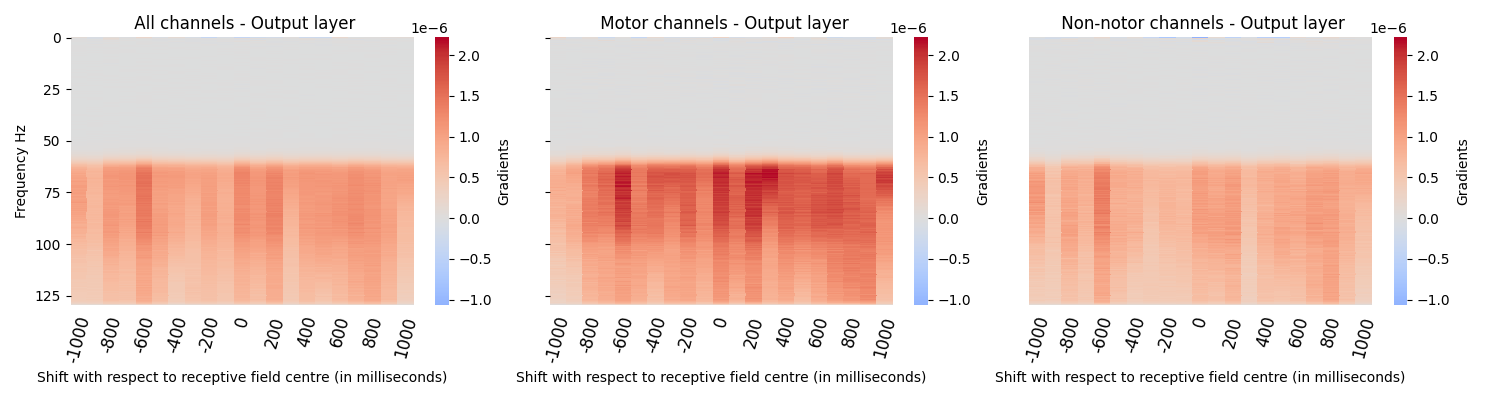
\includegraphics[width=0.85\linewidth]{img/appendix/C/hp-m/absVel/sbp0_hp_m_shift_gradients_conv_classifier_all_kinds}
   \caption{}
   \label{fig:absVel-hp-shifting-grads-conv-classifier}
\end{subfigure}

\caption[]{Gradients of the different CNN architectures decoding absolute velocity from the high-passed dataset when gradually shifting the predicted time-point (see Section~\ref{subsec:shifting-the-predicted-time-point-across-receptive-field}. \textbf{(a)} shows gradients of the convolutional layer in the second block; \textbf{(b)} shows gradients of the convolutional layer in the third block; \textbf{(c)} shows gradients of the fourth convolutional block; \textbf{(d)} shows gradients of the last convolutional layer - the output layer. All channels include channels that do not belong to motor neither non-motor channel sets. See Section \ref{subsec:ieeg-data-preprocessing}}
\label{fig:absVel-hp-shifting-grads}
\end{figure}